\begin{center}
    \textsc{\huge CANDIDATURA}\\[0.75cm] 
    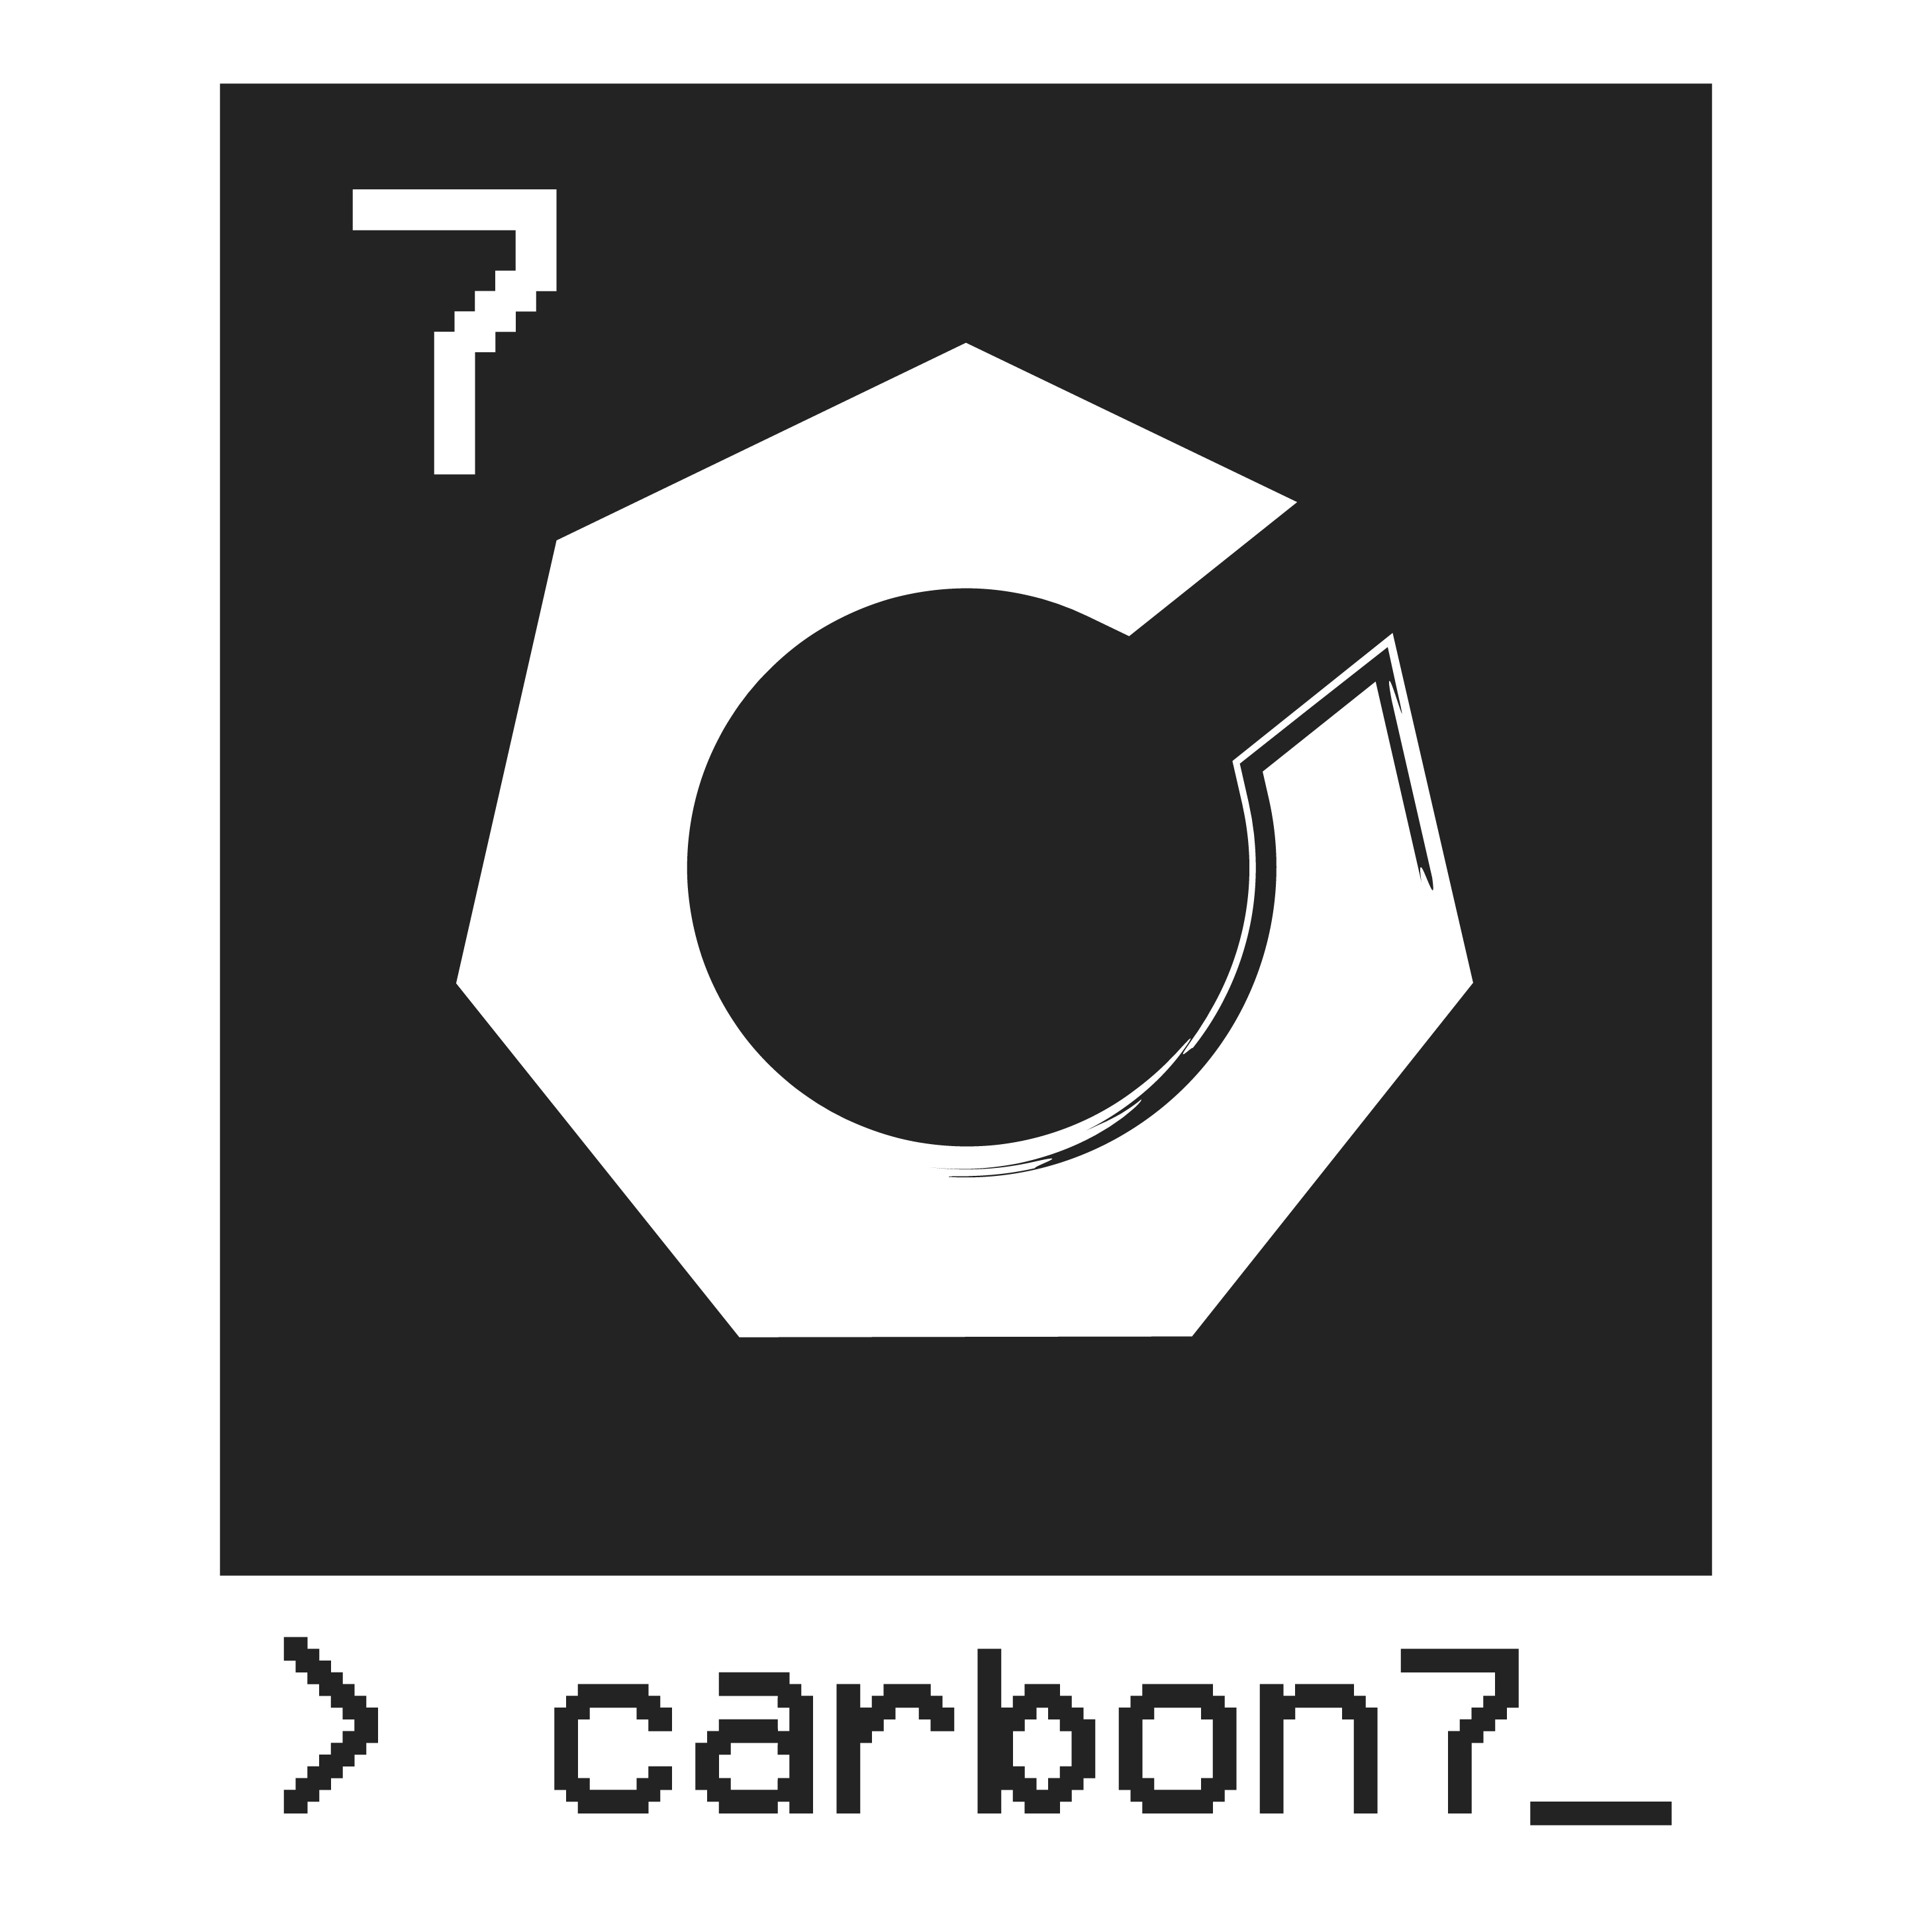
\includegraphics[scale=0.25]{res/images/carbon7_small_logo-07.png}\\[1cm]
    \textsc{\Large Carbon7team}\\[0.3cm]
    \text{\large carbon7team@gmail.com}\\[0.5cm]
    {\large 18 Novembre 2021}\\[0.5cm]
    \text{\large Repository github: \href{https://github.com/carbon7team}{\large \underline{Carbon7team}}}\\[0.5cm]

    \HRule \\[0.4cm]
    {\huge \bfseries Presentazione Candidatura}\\[0.2cm]
    \HRule \\[1cm]
    \begin{tabular*}{0.43\textwidth}{@{\extracolsep{\fill}} p{3.5cm} p{6cm} }
        \hline
        & \\
        \textbf{Componenti} & \textbf{Committente} \\
        & \\
        \hline
        & \\
        Filippo Brugnolaro  & Tullio Vardanega  \\[0.1cm]
        Adnan Latif Gazi    &                   \\[0.1cm]
        Matteo Noro         &                   \\[0.1cm]
        Andrea Polato       &                   \\[0.1cm]
        Damiano D'Amico     &                   \\[0.1cm]
        Leonardo Speranzon  &                   \\[0.1cm]
        Marco Odinotte      &                   \\
        & \\
        \hline
    \end{tabular*}
    \\[0.7cm]
    \textbf{Sommario}\\
    Candidatura al capitolato proposto da \copyright Socomec\\
    con motivazioni della scelta e dichiarazione d'impegno
\end{center}    
\newpage